\chapter{FFmpeg Interactions}%
\label{cha:ffmpeg_interactions}

Cinelerra-GG uses ffmpeg for decoding and encoding media, thus there are many opportunities available to manipulate options.

\section{FFmpeg Early Probe Explanation}%
\label{sec:ffmpeg_early_probe_explanation}

When you open media, a series of libraries and codec functions are used to \textit{probe} the data, to see if it can determine the type of file format and codec parameters needed to correctly decode the file.  If ffmpeg probes early --- \texttt{Try FFMpeg first} is in effect for the FF button --- it will usually find some way to try to decode just about any contemporary media file.  But there are some times that the built in codecs are actually a better choice.  A lot of this may fall into the category of personal preference.  For example, some may prefer the mpeg library in the Cinelerra code over the ffmpeg code because it has more decoding capability and seems to be more robust when the media is damaged.  In that case you will want the FF button to read \texttt{Try FFMpeg last}.

To summarize, if ffmpeg probes early, you will never get to use the built in libraries, and if you want to skip over buggy old libraries, use ffmpeg early probe enabled so that the newest code will be tried first.
The FF button is located in the upper right hand corner of the main window.

When the icon is red, ffmpeg probes early is enabled and you will see it reads
 \textit{Currently: Try FFMpeg first} when moving over the FF button in the upper 
right hand corner of the screen.  When the icon is black, ffmpeg probes early is disabled so that 
ffmpeg probes late and it reads \textit{Currently: Try FFMpeg last}.  The initial default state of 
the icon is on, that is, ffmpeg probes first. Suggestion is to leave it on except in a few special 
cases where it may be better to have early probes disabled.  When you mouse over the main menu FF 
toggle button, the text displays ffmpeg's \textit{Currently} set position.  Just left mouse click to change to the other setting.
The ffmpeg early probe state is saved between sessions and is also affected by choices made in Probe Order (refer to section 4 - Probe Order when Loading Media). It is important to note that the various file indexes may need to be rebuilt if you change which codec is being used to decode the file.  There is a warning popup to remind you when you change the default ffmpeg early probe state (unless you have checked the box to no longer show the warning).  You can easily rebuild the index for a specific media file by going to the Resources window, right mouse click on that media, and choose \texttt{Rebuild Index} from the popup choices.

Figure~\ref{fig:ff} shows (1) reddish colored FF in upper right hand corner of main window indicating
that ffmpeg early probes is enabled; (2) \textit{Try FFMpeg last}  indicator message for ffmpeg early probes enabled (note that the color is different because you highlighted the icon); and (3) black colored FF indicates ffmpeg will be used last and you are changing the behavior so that Cinelerra warns you accordingly.

\begin{figure}[htpb]
    \centering
    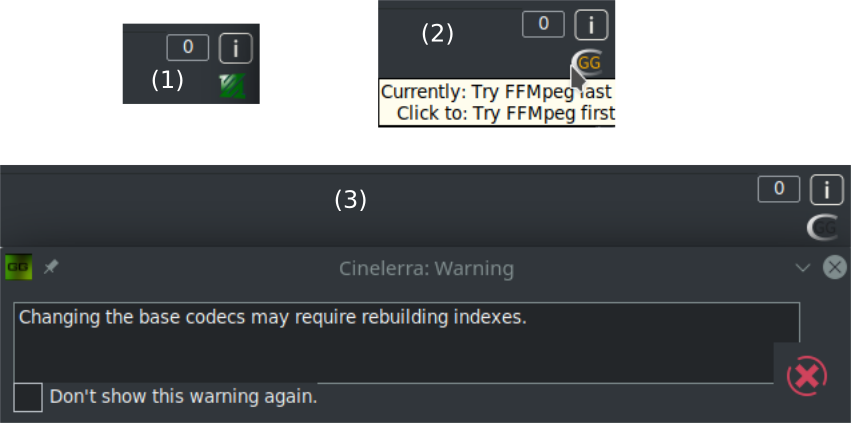
\includegraphics[width=0.7\linewidth]{images/ff.png}
    \caption{The three colors of \textit{Probe}}
    \label{fig:ff}
\end{figure}

\section{How to Create FFmpeg Options Files}%
\label{sec:create_ffmpeg_options_files}

This section describes how the FFmpeg options files work for decoding and encoding and goes into great detail.  It will make more sense if you look at Cinelerra's ffmpeg config directory and the Cinelerra menus at the same time.  
It is meant to include everything necessary for complete understanding.  You will be able to personalize your own options files without knowing all of the information included below if you know the basics.  The word encoding is used interchangeably with the word rendering.
The possible combinations for ffmpeg options files are literally combinatorial --- that is a lot (factorial!).  The allowed media file format / codec choices are much more flexible than you might realize.  When the ffmpeg design was initially added, some parameter files which describe the choices which the program uses had to be created.  There are way too many to enumerate in the deliverable Cinelerra package.  Some quite detailed information for how ffmpeg options work is given here and hopefully, enough basics for simple understanding.  It may all seem complicated at first, but will become obvious.

\subsection{File naming convention}%
\label{sub:file_naming_convention}

In Cinelerra's ffmpeg configuration directory you will see files as listed and described below.  File type and extension names are the key for Cinelerra's use of ffmpeg.  Basically the \texttt{.opts} file extension represents options; \texttt{.dfl} represents defaults; and all the rest are media types.  For example one media type is quicktime so that \texttt{*.qt} file names would be the \textit{quicktime} choices.  In the file names below, \texttt{ext} refers to a set of files with file names matching the \texttt{*.ext} file extension.  And \texttt{typ} refers to a type of format / codec combination used, that is, the media type.

In the ffmpeg configuration directory there are a series of options files used when encoding or decoding audio or video.  They are read in the order from top to bottom and only the files needed for the current operation are added to the active configuration.

\begin{center}
    \small
    \begin{tabular}{l l}
        \toprule
        ffmpeg/ffmpeg.opts & global ffmpeg options, always used \\
        ffmpeg/decode.opts & global decoder options, used when opening existing files for decoding \\
        ffmpeg/encode.opts & global encoder options, used when creating new files for encoding \\
        ffmpeg/audio/audio.opts & audio encoder options, used when creating audio streams \\
        ffmpeg/video/video.opts & video encoder options, used when creating video streams \\
        ffmpeg/plugin.opts & parameters for ffmpeg filters as audio/video plugins \\
        \bottomrule
    \end{tabular}
\end{center}

\paragraph{Decoder options:} Normally, only \texttt{ffmpeg.opts} and \texttt{decode.opts} are used when reading/decoding files, but may be specialized if a \texttt{<path>/media.opts} exists for a given \texttt{<path>/media.ext} file.  For example, if you want to only fail on fatal errors and to always use the video filter, edgedetect, when working with your media file \texttt{dreaming.y4m}, then create a file \texttt{dreaming.opts} in the same directory with the contents of \texttt{loglevel=fatal} on the first line and \texttt{video\_filter=edgedetect} on the next.  These specialized settings will override the defaults.  The fatal loglevel is especially handy for lesser quality media.

\paragraph{Encoder Options:} Within the audio/video subdirectories of the first level ffmpeg directory, the \texttt{typ.ext} files are for encoder (rendering) setups.

\begin{center}
    \begin{longtable}{l p{23em}}
        \toprule
        ffmpeg/audio & directory of audio encoder settings \\
        \midrule
        audio.opts & options used by all audio encoders \\
        typ1.ext, typ2.ext, … & are all *.ext type choices for encoding audio \\
        ext.dfl & contains the default selection used when ext is first selected \\
        \midrule
        ffmpeg/video & directory of video encoder settings \\
        \midrule
        video.opts & options used by all video encoders \\
        typ1.ext, typ2.ext, … & are all *.ext type choices for encoding video \\
        ext.dfl & contains the default selection used when ext is first selected \\
        \midrule
        ffmpeg/format & presets needed to initialize audio / video formats \\
        \bottomrule
    \end{longtable}
\end{center}

\subsection{Option File Format / Content}%
\label{sub:option_file_format_content}

For the option files a specific format must be followed in creating the file content.
In \texttt{typ.ext} encoder parameter files, the first line is defined as:

\begin{lstlisting}[language=bash,numbers=none]
      muxer codec
(or) 	muxer codec | bitstream filter [ bitstream filter options ]
\end{lstlisting}

where the | represents piping the codec data through the bitstream filter. The rest of the lines in the file should look as follows:

\begin{lstlisting}[language=bash,numbers=none]]
      # in column one is a comment
      id1   value1
(or)	id2 = value2
\end{lstlisting}

Only one equals sign is allowed and it is just for readability.  There may be any number of id / value pair lines in a media definition, including zero. A typical line might be:

\begin{lstlisting}[language=bash,numbers=none]]
      bitrate 4000000
(or)	bitrate = 5000000
\end{lstlisting}

There are 4 special id's recognized by Cinelerra which cause special processing.  They are:

\begin{description}
    \item[duration] overrides the probe duration when opening media for decoding
    \item[video\_filter] adds a video stream filter, eg. edgedetect,\dots at the stream level
    \item[audio\_filter] adds an audio stream filter, eg. echo,\dots at the stream level
    \item[loglevel] sets the library logging level, as quiet, panic, \dots verbose, debug
\end{description}

All other id's should be in the ffmpeg documentation, and correspond to the global, muxer, and codec option names and values used by ffmpeg.  For example to set the aspect ratio to 4:3, use:

\begin{lstlisting}[language=bash,numbers=none]]
aspect 4:3
\end{lstlisting}

Below shows an example:  \texttt{decode.opts} which is used when the ffmpeg decoder is initialized.

\begin{lstlisting}[language=bash,numbers=none]]
# apply at init decode
loglevel=fatal
formatprobesize=5000000
scan_all_pmts=1
threads=auto
\end{lstlisting}

The encoder options you see in the Cinelerra menus depend on the files in these directories, \textsc{NOT THE CODE}.  If you add files, you will get to use more variety.

In the \textit{cinelerra} directory, which contains the ffmpeg configuration folder, there are the choices the program uses.  When you open an ffmpeg format popup dialog, the listbox contains all of the codec types which are identified by the file.ext extensions.  Decoding has only a few options, since the ffmpeg file probes determine most of the options by looking at the media being opened, but encoding media requires a lot of setup.  Below are some of the folders and files used to determine the configurations used by ffmpeg to decode and encode files.

These extensions create audio / video media classes:

\texttt{dvd \quad  m2ts \quad  mkv \quad  mp3 \quad  mp4 \quad  mpeg  \quad qt \quad  pro}

which become the choices in the render pulldown menu.

So if you want to create a \textit{mov} codec class, add two new files to the ffmpeg configuration directory:

\texttt{audio/aud.mov}  and  \texttt{video/vid.mov}

Now you will see this as what you can choose in the rendering choices for ffmpeg.
Inside the file you will see that the first line is special.  It is the muxer and codec.  For example:

\begin{lstlisting}[language=bash,numbers=none]]
h264     libx265
\end{lstlisting}

The contents may be something like:

\begin{lstlisting}[language=bash,numbers=none]]
# <path>/video/vid.mov 
mp4 libx265
bitrate 4000000
\end{lstlisting}

This will code an \texttt{mp4} formatted file using the \texttt{lib264} codec encoder.

For audio and video together, the mux format must agree between the aud.mov and vid.mov files when they are to be used together.  The stream muxer must be the same for all the streams in the file being written.
for example:

\begin{lstlisting}[language=bash,numbers=none]]
# <path>/audio/aud.mov
mp4 pcm_mulaw
\end{lstlisting}

This will create \textit{mp4} media using audio format \texttt{pcm\_mulaw} coding.

Both the audio and the video are using \textit{mp4} mux format, and so there will be 2 streams:
\begin{enumerate}
    \item x265 video
    \item pcm\_mulaw audio
\end{enumerate}

When the menu popup is created, there may be many choices for that class type, so you may want defaults.  That can be specified as:

\texttt{audio/<class>.dfl}  and  \texttt{video/<class>.dfl}

\begin{lstlisting}[language=bash,numbers=none]]
# audio/mov.dft
aud.mov
\end{lstlisting}

\begin{lstlisting}[language=bash,numbers=none]]
# video/mov.dft =
vid.mov
\end{lstlisting}

The above will be the default choice when the menu opens.  

When you see problems in using the new options files you have created and put into place, add the following line to \texttt{ffmpeg/encoder.opts}:

\begin{lstlisting}[language=bash,numbers=none]]
loglevel=verbose
\end{lstlisting}

sometimes that will be enough to see what has caused a failure, or even catch unexpected results.

There is an \textsc{EXCEPTION} to all of the above because of a conflict between ffmpeg and the x264 person making the detection of default ffmpeg settings terminate with an error.  If you get this error, you must workaround this termination by including parameters that don't match $5$ or more of the normal expected values.  So you just have to change a few parameters to avoid the probe detection.  Here is an example where you will notice the \texttt{x264-params} line tweaking values to throw off the detection/error termination code.

\begin{lstlisting}[language=bash,numbers=none]]
# <path>/ffmpegvideo/test.mp4
mp4 libx264
preset=slow
x264-params keyint=25:min-keyint=4:qpmin=3:qpmax=33:qp_step=4:merange=8
crf 20
\end{lstlisting}

For more examples, look around the ffmpeg directory for examples which may be close to what you are trying to use, and see if the parameters look usable. 

This is quite complicated, but that is because ffmpeg has a lot of parameters and history.  Good results are not that hard to create.  Initially you should mostly use the defaults.  
If you send any new options files to \href{mailto:cin@lists.cinelerra-gg.org}{cin@lists.cinelerra-gg.org}, it will be given consideration to being added to the baseline for future deliverables.

To get a listing of the current ffmpeg supported formats and codecs that can be made to work with Cinelerra, provided there are option files added, run the following commands.  This should be done from the <build>directory substituting the location of <build> where you have installed Cinelerra on your system and the ffmpeg may be a different version than $4.2$ as used below.  Then look at the output created in \texttt{/tmp/ff-formats.txt} and \texttt{codecs.txt}.

\begin{lstlisting}[language=bash,numbers=none]]
/<build>/cinelerra-5.1/thirdparty/ffmpeg-4.2/ffmpeg -formats > /tmp/ff-formats.txt
/<build>/cinelerra-5.1/thirdparty/ffmpeg-4.2/ffmpeg -codecs > /tmp/ff-codecs.txt
\end{lstlisting}

\subsection{Complete Options File Example}%
\label{sub:complete_options_file_example}

For illustrative purposes, here is an example of the options files that need to be added for using the ffmpeg \textit{ProRes 422} format. This makes it possible to transcode to \texttt{h264.mov} with FFmpeg retaining \textit{10-bit yuv422p} from the source to the target output video.

Add the file named  \texttt{./ffmpeg/audio/acc256k.pro} which contains the following lines:

\begin{lstlisting}[language=bash,numbers=none]]
mov aac
strict -2
b 256000
\end{lstlisting}

(Note that in the example above, even though the bitrate is set here to $256000$, it can be 	overridden by the render menu settings).

Add the file named \texttt{./ffmpeg/audio/pro.dfl} which contains the following lines:

\begin{lstlisting}[language=bash,numbers=none]]
acc256k.pro
\end{lstlisting}

Add the file named \texttt{./ffmpeg/video/prores.pro} which contains the following lines:

\begin{lstlisting}[language=bash,numbers=none]]
mov prores
profile=2
# lines of comments
\end{lstlisting}

Add the file named \texttt{./ffmpeg/video/pro.dfl} which contains the following lines:

\begin{lstlisting}[language=bash,numbers=none]]
prores.pro
\end{lstlisting}

Then to use and to get 10 bit depth and preserve depth from decode to encode:

\begin{enumerate}
    \item load media
    \item use settings$\rightarrow$format to set the frame rate, sample rate/channels, aspect ratio, 
    color model = rgb\_float or rgba\_float if blending
    \item press \texttt{Shift-R} and select FFmpeg format type \texttt{pro}
    \item select target path
    \item check \texttt{OK}, and watch for messages in the terminal window
\end{enumerate}

\subsection{Viewing \& Modifying FFmpeg Format Options inside Cinelerra}%
\label{sub:viewing_modifying_ffmpeg_cinelerra}

There are thousands of options for using ffmpeg.  Now it is possible to \textit{view} the available options for a particular video and audio choice by using the \textit{wrench icon} and then clicking on the \textit{view} box.  FFmpeg has to be the selected file format for this feature to be visible.  It makes it a lot easier since only the applicable options show up as opposed to everything that ffmpeg can do.  These options are just \textit{Hints} and some may be missing due to the way that ffmpeg options are coded --- Cinelerra shows the option data ffmpeg has exposed.

As an example, instead of reading the entire 264 library information, you only have to look at the shown available options.  Both the video and the audio are browsable. The options visible in the \textit{Audio/Video Preset} textbox are the final values which are used when rendering once you have checked \texttt{OK}.  For assistance in choosing the options you want, use the view popup to see the objects that go with the selected format tool, highlight the option, modify the parameter value in the box at the top of the \textit{Options} window based on what you want, and then click apply.  Updated parameter values or new parameters will be appended at the bottom.  Note that when you highlight an option, a tooltip will show up when available in the lower right hand corner which describes the option.  Also note that the Format and Codec types are shown on the top line of the Options window.

Parameters exist in 3 layers: ffmpeg, codec, and an interface layer.  You can apply parameters to each layer.  The top 2 layers are accessed with the Kind popup menu. The ffmpeg layer is topmost, and is selected as Kind: ffmpeg.  It can specify many of the more common parameters, such as the bitrate, quality, and so on.  The middle layer is selected as Kind: codec.  These options can specialize your choices, and frequently includes presets and profiles useful for coding well known parameter sets, like \texttt{profile=high422}, \texttt{preset=medium}, or \texttt{tune=film}, etc.   The interface layer may or may not be available.  It is usually accessible only by an \textit{opts} parameter, like \texttt{x264-params key=value:key=value:\dots}  These options are passed directly to the low level codec library.

Figure~\ref{fig:video-preset} shows \textit{ffmpeg} video as the Kind. Note the x264opts (should actually be x264-params now) in the Video Preset window immediately below.

\begin{figure}[htpb]
    \centering
    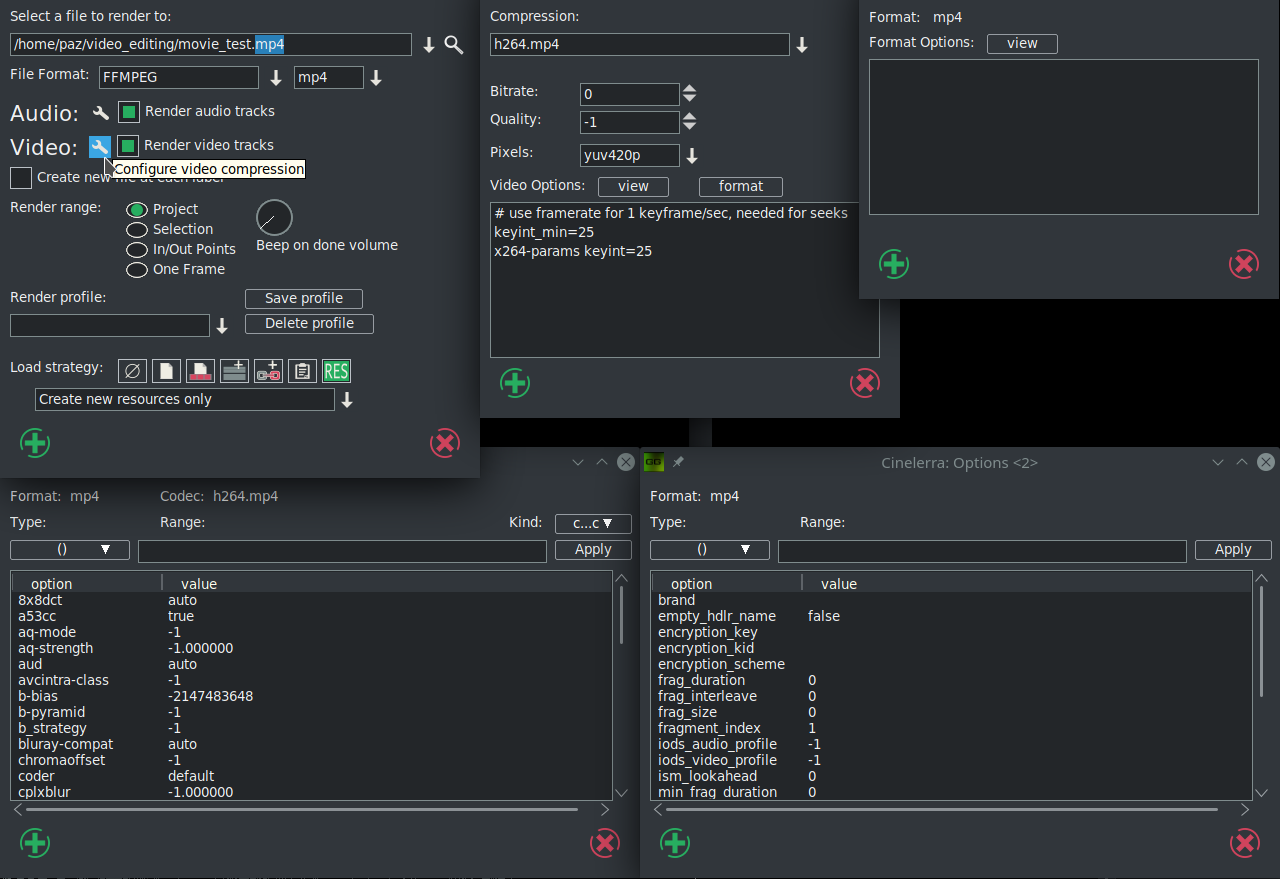
\includegraphics[width=0.8\linewidth]{images/video-preset.png}
    \caption{FFmpeg wrench, video preset and view options}
    \label{fig:video-preset}
\end{figure}

Figure~\ref{fig:audio-preset02} shows \textit{ffmpeg} video for the Kind. Note the yellow tooltip in the lower right hand corner describing the highlighted option.  Also note the allowed \textit{Range} values above the box provided for keyins.

\begin{figure}[htpb]
    \centering
    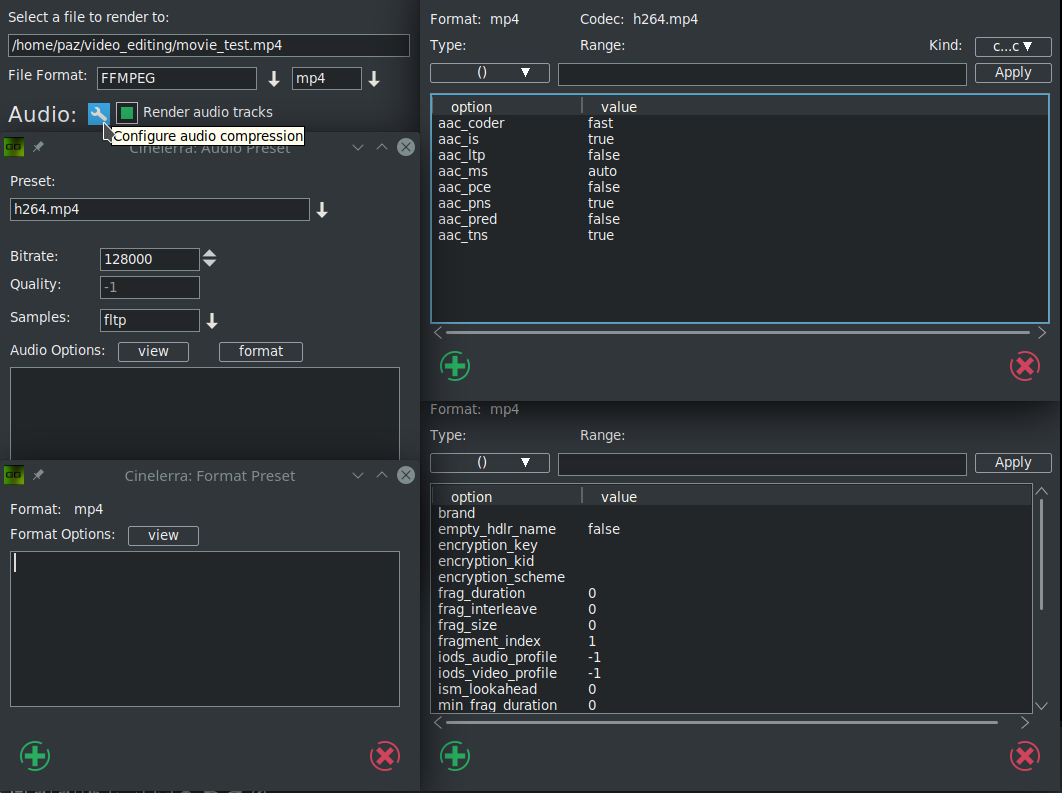
\includegraphics[width=0.8\linewidth]{images/audio-preset02.png}
    \caption{FFmpeg wrench, audio preset and view options}
    \label{fig:audio-preset02}
\end{figure}

\section{The FFmpeg Image2 Streams}%
\label{sec:ffmpeg_image2_streams}

Another feature gained from using ffmpeg in Cinelerra takes advantage of what is being referred to as the \textit{\%d trick}.  This trick uses the ffmpeg muxer image2 and a filename template to create a series of image files of a given type.  A specific example is described below.

To encode a series of $48$ bit tiff output image files, add a file to the cinelerra data ffmpeg/video subdirectory as in:

\begin{lstlisting}[language=bash,numbers=none]]
# \dots/ffmpeg/video/tiff.dfl
tiff48.tif
\end{lstlisting}

Then create an ffmpeg video encoder parameters file in the same directory:

\begin{lstlisting}[language=bash,numbers=none]]
# \dots/ffmpeg/video/tiff48.tiff
image2 tiff
pixel_format=rgb48
\end{lstlisting}

This will define a new ffmpeg encoder format which is a video image file format that uses the tiff codec for encoding, and a pixel\_format of \texttt{rgb48} (or a similar equivalent such as rgb48le).  Next load up your project and set up for a Render using File$\rightarrow$Render in the usual way.  Now the tricky part; the output file name should contain a \texttt{\%d} which will be the frame number used in the image output filename as in:  Select a file to render to  \texttt{/tmp/tiff\_images/img\%03d.tiff}.  You will get multiple files as output --- one for each frame!

The resulting directory of images can be opened for reading by simply opening the template path.  As in: File$\rightarrow$Load Files \texttt{/tmp/tiff\_images/img\%03d.tiff}.  You will notice a file named the same as the template, which has been automatically created, is empty, is needed, and has to remain with the set.

\section{Raw Input Opts File for Video/Audio}%
\label{sec:raw_input_opts_video_audio}

Raw video is not affected by decoding on read in.  This makes it very attractive to provide raw image data for editing and rendering media.  A wide variety of raw formats are available via the ffmpeg file interface.  To load media in a raw format, select \texttt{try ffmpeg first} and create an accompanying \textit{opts} file.  The opts files must be in the same directory as your media, with the same base name, and the \texttt{.opts} extension.  The opts file contents should reflect your video setup.  An example follows:

\begin{lstlisting}[language=bash,numbers=none]]
# Video file name:    /tmp/buddy.mov
# Opts file name:     /tmp/buddy.opts
# Contents of opts file:

format=rawvideo
codec=rawvideo
video_size=352x240
pixel_format=yuv420p
duration=90.25
\end{lstlisting}

\section{FFmpeg Items of Note}%
\label{sec:ffmpeg_items_note}

\begin{description}
    \item[Quality Option when rendering:] FFmpeg responds variably to the quality option in the render option but seems to respond well to bitrate. The subranges used by quality even seem to vary somewhat depending on how old the codec is. Some use $0$ to $35$, some use $0$ to $500$ or so.  The quality is supposed to cause the codec to output data until the noise level is below a limit determined by the quality setting. Your specific results may vary.
    \item[Previous Changes when rendering:] With ffmpeg there are 2 cases that the defaults will be used.  The first time when you have nothing set up and any other time when you reset the render File Format in the Render Menu.  Otherwise with ffmpeg, if you change a video compression type for the render (for example \texttt{h264.mp4} to \texttt{h265.mp4}), the settings will be from the previous session settings.
    \item[Outstanding Issues with ffmpeg:] There are some problems that need to be addressed by the ffmpeg developer group that adversely affect Cinelerra.  These are stated below with the hopes that that group will fix them as time permits.
    \begin{itemize}
        \item Make all the default parameters operational.  When they are not, the Cinelerra plugins can't be initialized since the initial state of the filter is not operational.  If that is not possible, then provide a set of nominal parameters for each plugin, so that they can be used as the plugins initial default state.
        \item Make the filter config function project the new parameter data into the filter function at any point
        during filter operation.  This is so that continuous updates can be done as the plugin operates.
        \item Improve seek codec restarts.  The past predictor must be reset or reconstructed after a seek.  The  only documented way to seek is open/seek/play.  Reopening the format layer is very expensive.
    \end{itemize}
\end{description}
